\begin{figure}[!htbp]
  \centering
  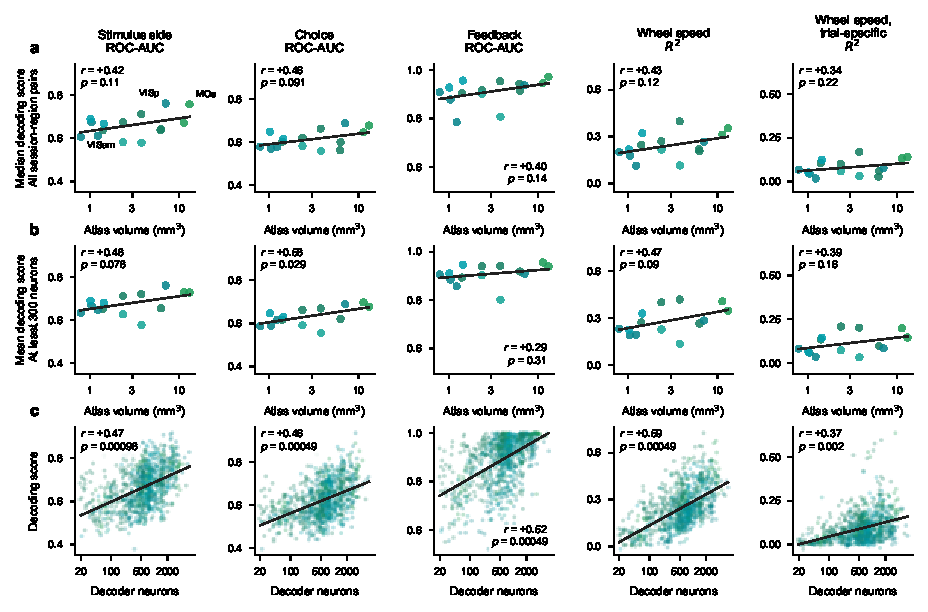
\includegraphics[width=\linewidth,height=0.8\textheight,keepaspectratio]{figures/meso_size_scaling.pdf}
  \caption{Mesoscope decoding versus region volume and neuron count. \textbf{a} Bilateral Beryl region volume from the 25-micron Allen CCF atlas versus the median score across sessions in that region (one dot per region, 15 regions). Scores are the mesoscope all-neuron decoding scores from \figref{region_variance}a. Two-sided $p$-values use 9,999 shuffles of volumes across regions. Dots in all panels use Allen atlas colours for their Beryl regions. \textbf{b} Atlas volume versus the mean score per region, using only session--region pairs with at least 300 decoder neurons. Each region with an eligible pair contributes one dot. The same volume permutation test is used. \textbf{c} Number of neurons used by the decoder versus score, with one dot per session and region. The two-sided slope test flips the signs of the null score contributions by mouse, keeping each mouse's observations together (12 mice). All rows use log-scaled horizontal axes. Lines are least-squares fits and $r$ is Pearson correlation with the log predictor. Displayed $p$-values are unadjusted. Holm-adjusted values across all 15 tests are in the accompanying CSV.}
  \label{fig:meso_size_scaling}
\end{figure}
